\documentclass[12pt,letterpaper]{article}
\usepackage{graphicx,textcomp}
\usepackage{natbib}
\usepackage{setspace}
\usepackage{fullpage}
\usepackage{color}
\usepackage[reqno]{amsmath}
\usepackage{amsthm}
\usepackage{fancyvrb}
\usepackage{amssymb,enumerate}
\usepackage[all]{xy}
\usepackage{endnotes}
\usepackage{lscape}
\newtheorem{com}{Comment}
\usepackage{float}
\usepackage{hyperref}
\newtheorem{lem} {Lemma}
\newtheorem{prop}{Proposition}
\newtheorem{thm}{Theorem}
\newtheorem{defn}{Definition}
\newtheorem{cor}{Corollary}
\newtheorem{obs}{Observation}
\usepackage[compact]{titlesec}
\usepackage{dcolumn}
\usepackage{tikz}
\usetikzlibrary{arrows}
\usepackage{multirow}
\usepackage{xcolor}
\newcolumntype{.}{D{.}{.}{-1}}
\newcolumntype{d}[1]{D{.}{.}{#1}}
\definecolor{light-gray}{gray}{0.65}
\usepackage{url}
\usepackage{listings}
\usepackage{color}

\definecolor{codegreen}{rgb}{0,0.6,0}
\definecolor{codegray}{rgb}{0.5,0.5,0.5}
\definecolor{codepurple}{rgb}{0.58,0,0.82}
\definecolor{backcolour}{rgb}{0.95,0.95,0.92}

\lstdefinestyle{mystyle}{
	backgroundcolor=\color{backcolour},   
	commentstyle=\color{codegreen},
	keywordstyle=\color{magenta},
	numberstyle=\tiny\color{codegray},
	stringstyle=\color{codepurple},
	basicstyle=\footnotesize,
	breakatwhitespace=false,         
	breaklines=true,                 
	captionpos=b,                    
	keepspaces=true,                 
	numbers=left,                    
	numbersep=5pt,                  
	showspaces=false,                
	showstringspaces=false,
	showtabs=false,                  
	tabsize=2
}
\lstset{style=mystyle}
\newcommand{\Sref}[1]{Section~\ref{#1}}
\newtheorem{hyp}{Hypothesis}

\title{Problem Set 4}
\date{Due: April 12, 2024}
\author{Applied Stats II}


\begin{document}
	\maketitle
	\section*{Instructions}
	\begin{itemize}
	\item Please show your work! You may lose points by simply writing in the answer. If the problem requires you to execute commands in \texttt{R}, please include the code you used to get your answers. Please also include the \texttt{.R} file that contains your code. If you are not sure if work needs to be shown for a particular problem, please ask.
	\item Your homework should be submitted electronically on GitHub in \texttt{.pdf} form.
	\item This problem set is due before 23:59 on Friday April 12, 2024. No late assignments will be accepted.

	\end{itemize}

	\vspace{.25cm}
\section*{Question 1}
\vspace{.25cm}
\noindent We're interested in modeling the historical causes of child mortality. We have data from 26855 children born in Skellefteå, Sweden from 1850 to 1884. Using the "child" dataset in the \texttt{eha} library, fit a Cox Proportional Hazard model using mother's age and infant's gender as covariates. Present and interpret the output.


\begin{lstlisting}[language=R]

# Using the child dataset 

data(child)

child_surv <- with(child, Surv(enter, exit, event))

# fit a Cox Proportional Hazard model 
cox <- coxph(child_surv ~ sex + m.age, data = child)
summary(cox)

# check fit
drop1(cox, test = "Chisq")
stargazer(cox, type = "text")

\end{lstlisting}

\newpage
\noindent Results are as follows:

\begin{lstlisting}[language=R]
> stargazer(cox, type = "text")

================================================
Dependent variable:    
---------------------------
child_surv         
------------------------------------------------
sexfemale                     -0.082***         
(0.027)          

m.age                         0.008***          
(0.002)          

------------------------------------------------
Observations                   26,574           
R2                              0.001           
Max. Possible R2                0.986           
Log Likelihood               -56,503.480        
Wald Test                22.520*** (df = 2)     
LR Test                  22.518*** (df = 2)     
Score (Logrank) Test     22.530*** (df = 2)     
================================================
Note:                *p<0.1; **p<0.05; ***p<0.01
	
\end{lstlisting}

\begin{lstlisting}[language=R]
	
	> exp(-0.082)
	[1] 0.921272
	> exp(0.008)
	[1] 1.008032
	
\end{lstlisting}

\vspace{2.25cm}

\noindent \textbf{Interpretation}: There is a 0.082 decrease in the expected log of the hazard for female babies compared to 
male, holding mother's age constant. There is a 0.008 increase in the expected log of the hazard for babies of mothers as they age by a year, holding sex constant.\\

\noindent By exponentiating the parameter estimates to obtain hazard ratios, we find that the hazard ratio of female babies is 0.92 that of male babies, i.e. female babies are less
likely to die (92 female babies die for every 100 male babies; female deaths are 8 per cent lower, etc.)


\newpage

\noindent Presenting the results:

\begin{lstlisting}[language=R]
cox_fit <- survfit(cox)
autoplot(cox_fit)
\end{lstlisting}

\begin{figure}[htbp]
	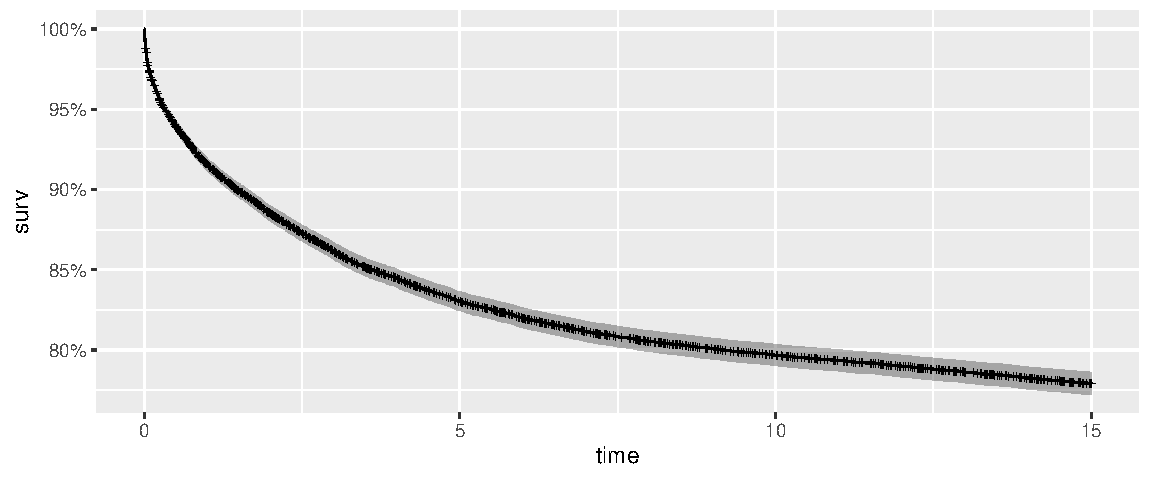
\includegraphics[width=1\linewidth]{Rplot}
	\caption{Hazard Function Results}
	\label{fig:rplot}
\end{figure}

\vspace{1cm}

\noindent We can also visualise the cumulative hazard function.

\begin{lstlisting}[language=R]
plot_COXPH <- coxreg(child_surv ~ sex + m.age, data = child)
plot(plot_COXPH)
\end{lstlisting}

\begin{figure}[htbp]
	\centering
	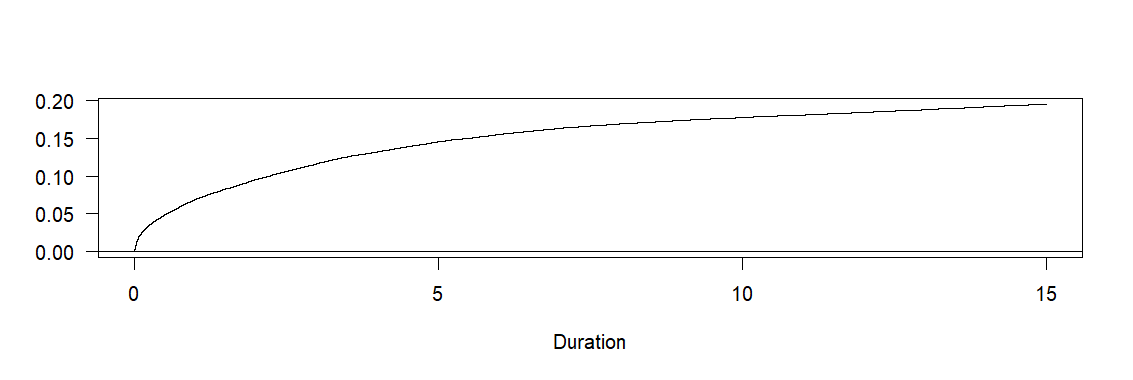
\includegraphics[width=1\linewidth]{Rplot05cumulative}
	\caption{Cumulative Hazard Function}
	\label{fig:rplot05cumulative}
\end{figure}

\newpage
\noindent The following plot provides a visualisation of the difference across genders, using an average age for the mother.

\begin{lstlisting}[language=R]

newdat <- with(child, 
data.frame(
sex = c("female", "male"), m.age = rep(mean(m.age,na.rm = TRUE, 2))
)
)

# using an average age
fit <- survfit(cox, newdata = newdat)

plot(survfit(cox, newdata = newdat), xscale = 1,
conf.int = T,
ylim = c(0.75, 1),
col = c("red", "blue"),
xlab = "Time",
ylab = "Survival proportion",
main = "")
legend("bottomleft",
legend=c("Male", "Female"),
lty = 1, 
col = c("red", "blue"),
text.col = c("red", "blue"))
\end{lstlisting}

\begin{figure}[htbp]
	\centering
	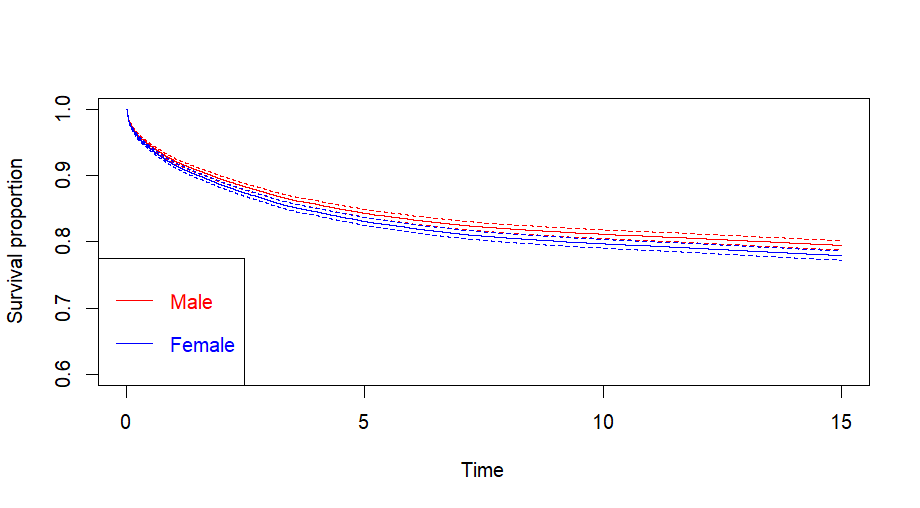
\includegraphics[width=1\linewidth]{Rplot03}
	\caption{Comparison of survival rate for male and female children using an average age for mothers}
	\label{fig:rplot01}
\end{figure}

\newpage
\noindent The following graph provides a visualisation of the difference in life expectancy for male and female children when the mother's age is at 20 and 40.

\begin{lstlisting}[language=R]
newdat20 <- with(child, expand.grid(m.age = c(20, 40), sex = c("male", "female")))

plot(survfit(cox, newdata = newdat), 
xscale = 0.30,
conf.int = TRUE,
ylim = c(0.75, 1),
col = c("red", "blue", "green", "black"), # Specify colors for each age group and sex
xlab = "Time",
ylab = "Survival proportion",
main = "")
legend("topright",
legend=c("Male (20)", "Male (40)", "Female (20)", "Female (40)"), 
lty = 1, 
col = c("red", "blue", "green", "black"),
text.col = c("red", "blue", "green", "black"),
cex = 0.6)

\end{lstlisting}

\begin{figure}[htbp]
	\centering
	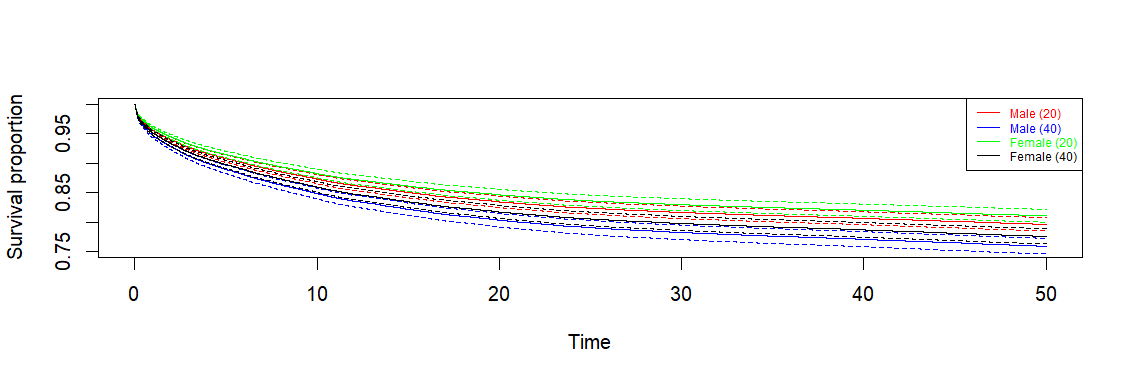
\includegraphics[width=1\linewidth, height=0.3\textheight]{Rplot04}
	\caption{Difference in life expectancy for children (male or female) when mother's age is at 20 or 40}
	\label{fig:rplot04}
\end{figure}

\end{document}